As previously mention our goal is to design and develop a tool that will asssist the user in gathering insightful data from unstructured data.
In order to achieve this target we decided to implement various methods into our project. Figure 1.1 displays the architecture designed for this specific project.  
\begin {figure} [h]
    \centering
    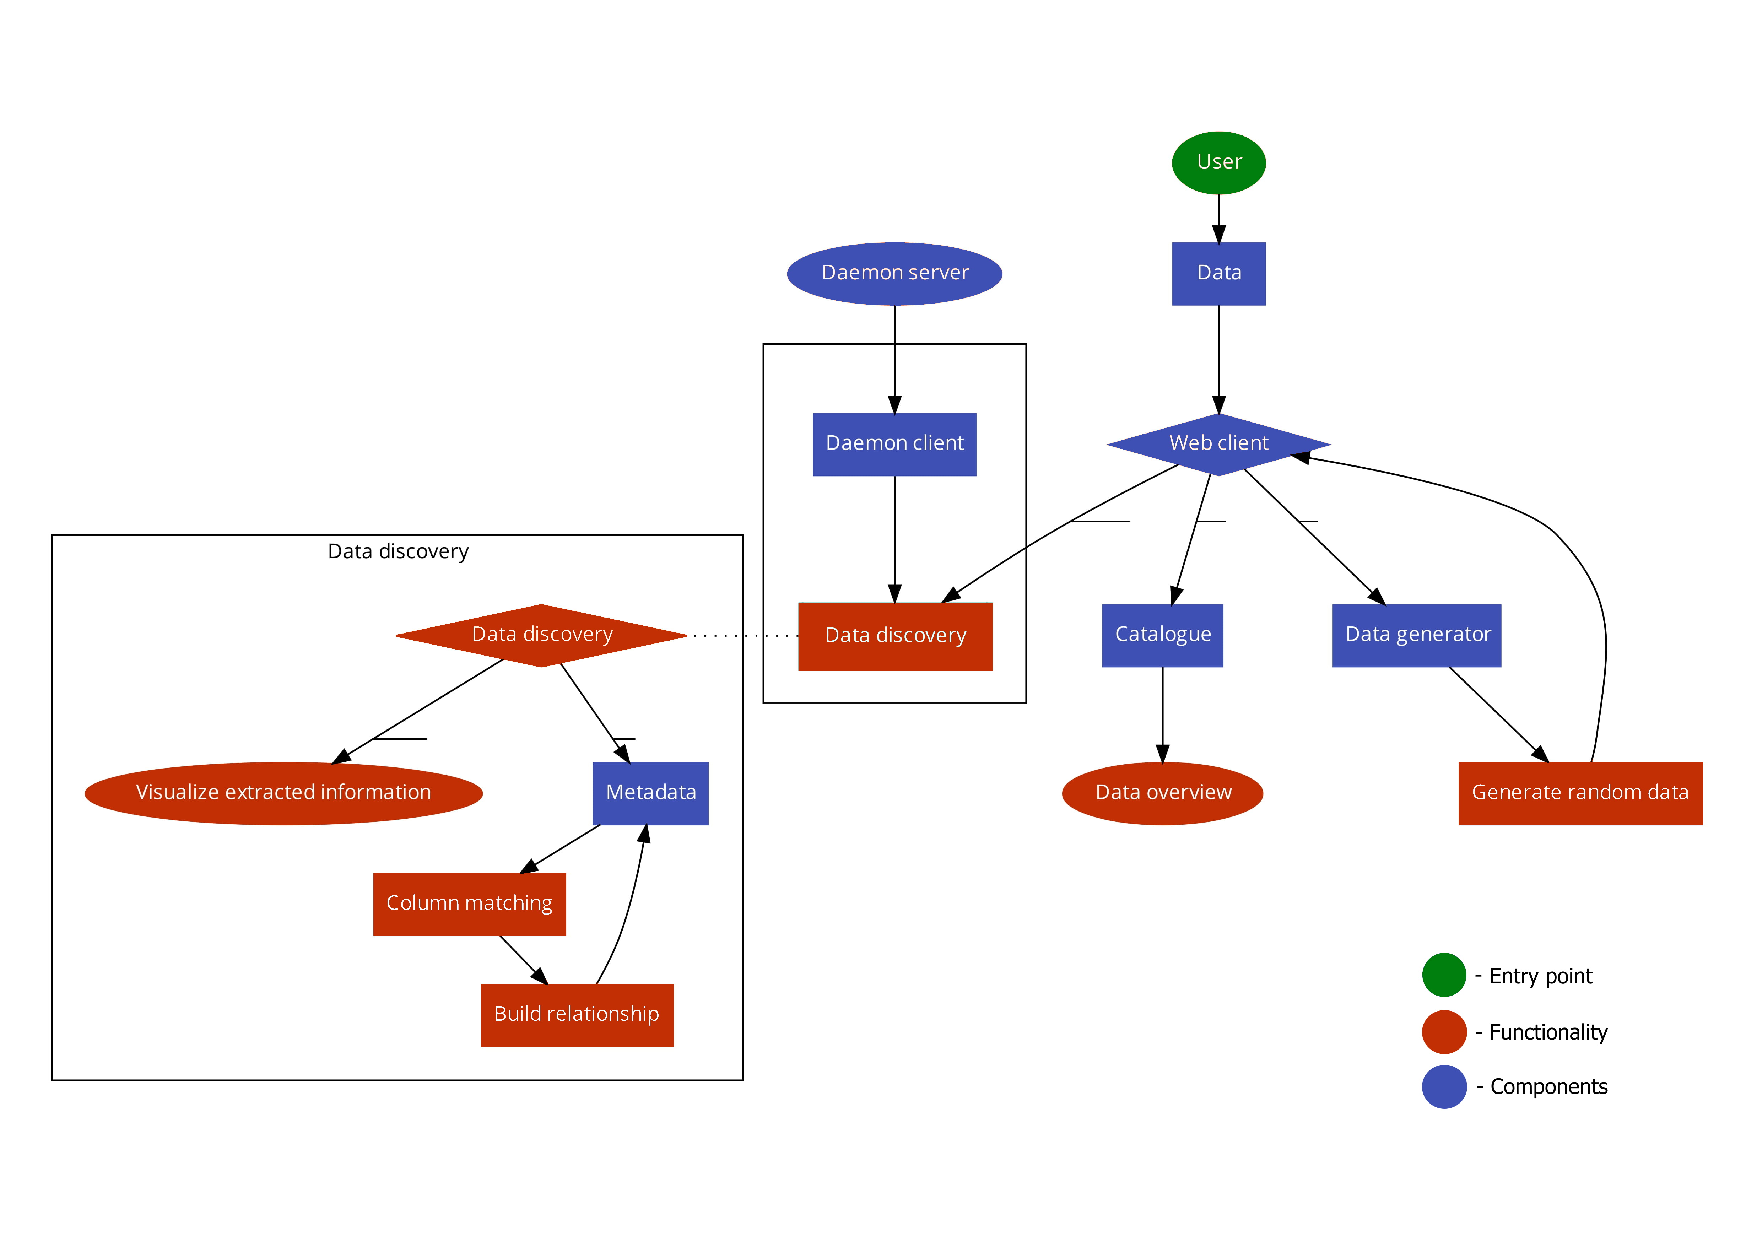
\includegraphics[width=16cm]{figures/architecture}
    \caption {Architecture}
    \label {fig:architecture_diagram}
\end{figure}
\vspace{5mm} %5mm vertical space
\subsection{Catalogue}
The catalogue offers an overview of the respective data. Further on, the catalogue will allow the user to see all the column relationship created by the metadata. Additionally, the user can also make changes to his data as for example, hiding unwanted columns.
\vspace{5mm} %5mm vertical space
\subsection{Data generator}
For testing purposes, we decided to create our own random data generator. We ended up with this decision because we believe that this will enable us to mold the data as we would like. Our data generator creates a simple table, and each column can be either numerical or categorical. As the title suggested, the data generated is random and doesn't replicate real life data. In order to combat performance issues, our approach was to abstract each column into its own class in order to build an arbitrary dataframe
on the specified columns. This choice enabled us to generate a big amount of "fake" data that can be easily used to further develop our main tool. An example of this data generator can be found on the web client.
\vspace{5mm} %5mm vertical space
\subsection{Data Discovery}
The goal of data discovery is to analyze and extract insight from the the provided data. The information gathered will be later used by metadata to build potential relationship between the columns in order to provide the user with insightful and relevant information about his data. Further on we can use this information to represent it in a more organized way. Our approach for data discovery was to take two files and try to match columns between those two files using multiple techniques.

\vspace{5mm} %5mm vertical space
\subsection{Metadata}
Metadata is one of the main features of our data discovery tool. The main point of metadata is to use all the information delivered by data discovery in order to create relationship between columns and files. In short, metadata is data that describes data.
\newline
Some of the objectives for our metadata were that we wanted our metadata to generate human readable information, but at the same time to also use a pre-existing format and have a low overhead. We also didn't want the users to be forced in installing a third party software in order to access the generated databases.
\newline

\clearpage
